\appendices

\section{Dataset Description}
\label{sec:dataset:description}

\PP{DARPA E3} The E3 dataset contains two kinds of threat actors: a nation-state actor and a common threat actor. The goal of the nation-state attacker is to steal proprietary information from the targeted company. Initially, the attacker intends to exploit the webserver hosted on FreeBSD, inject into the SSHD process, and then wait. At this point, the attacker monitors connections and network activity while residing on the FreeBSD host. Subsequently, the attacker targets and exploits the discovered hosts to exfiltrate proprietary data. The common threat attacker aims to steal Personal Identifiable Information (PII) for financial gain by deceiving targeted users into providing access to the network using spear phishing.

\PP{DARPA E5} The \darpa E5 dataset is more advanced than E3 in terms of attack complexity and data volume. The attackers' capabilities span the entire MITRE ATT\&CK~\cite{xiong2022cyber} adversarial lifecycle, from backdoors to exploit shellcode, from download to the execution of APT simulacra in-memory of the exploited process’s memory, from fingerprinting and surveying the target to exfiltrating sensitive data. Multiple variations of APTs and attack capabilities were delivered for Windows, Ubuntu, FreeBSD, and Android. The logs from E3 and E5 are documented under various scenario names, including Cadets, Trace, Theia, and ClearScope. The attacks in E3 were conducted on a single host per scenario, whereas E5 features three hosts per scenario, presenting a multi-host threat environment.

\PP{DARPA OpTC} The \optc dataset, another open-source resource from \darpa, encompasses a comprehensive collection of audit logs from an enterprise environment with 1,000 hosts. This dataset includes six days of benign system logs. Subsequently, attack logs span three days of system activities, featuring red team tactics such as initial compromises, privilege escalations, malicious software installations, and data exfiltration. Each attack day targeted different host machines.

 \section{RQ5: Comparison with existing FL solutions for heterogeneity.}
\label{sec:fedalternatives}

We conducted experiments to evaluate the efficacy of existing federated learning solutions that address data heterogeneity and the non-IID problem. Specifically, we examined FedProx~\cite{li2020federated} and FedOpt~\cite{asad2020fedopt}. FedProx mitigates client heterogeneity by adding a proximal term to the local loss function, penalizing deviations from the global model and thereby reducing the impact of statistical heterogeneity. In contrast, FedOpt uses a server-side optimizer to aggregate updates from distributed clients, enhancing convergence. We compared these techniques with standard FedAvg and the \Sys variant of FedAvg, which incorporates semantic harmonization and categorization based gnn ensemble learning. Table~\ref{fedoptprox} presents the evaluation results. Both FedProx and FedOpt outperform FedAvg; however, neither matches the performance of \Sys.

FedProx's penalty on global and local deviations focuses the model on patterns common across all clients, preventing it from learning client-specific patterns. Consequently, using this global model for anomaly detection on individual clients often yields numerous false alarms and poor detection performance. Moreover, while FedOpt can effectively aggregate model updates using an optimizer rather than simple averaging, updates that are highly disparate—a common scenario in system logs due to diverse client activities—cause FedOpt to fail in harmonizing the updates. As a result, it loses information on important benign patterns, leading to low precision and recall.

In contrast, our system employs an ensemble learning framework. First, it categorizes system patterns into standardized bins via process entity categorization. Next, \gnnshort submodels learn the data distribution within each bin. Submodels with similar learned distributions are then averaged, preventing the conflation of unique client patterns and improving precision. Moreover, our semantic vector harmonization reduces heterogeneity in the \gnnshort feature vectors, making the updates less disparate and improving model convergence in comparison to other techniques.


\begin{table}[!t]
  \centering
  \footnotesize
  \caption{Federated averaging algorithms comparison.}
  \setlength{\tabcolsep}{1.6pt}
  \begin{tabular}{cccccccccc}
    \toprule
    \multirow{2}{*}{\textbf{Methods}} & \multicolumn{3}{c }{\textbf{\optc}} & \multicolumn{3}{c }{\textbf{E3}} & \multicolumn{3}{c }{\textbf{E5}} \\
    \cmidrule(r){2-4} \cmidrule(r){5-7} \cmidrule(r){8-10}
    & {\bf Prec.} &  {\bf Rec.} & {\bf F-score} & {\bf Prec.}  & {\bf Rec.} & {\bf F-score} & {\bf Prec.}  & {\bf Rec.} & {\bf F-score} \\
    \midrule

    FedAvg & 0.36 & 0.99 & 0.53  & 0.73 & 0.99 & 0.84 & 0.76 & 0.98 & 0.86 \\
    FedProx & 0.48 & 0.95 & 0.64 & 0.79 & 0.98 & 0.87 & 0.82 & 0.95 & 0.88 \\
    FedOpt & 0.52 & 0.90  & 0.74 & 0.81 & 0.97 & 0.88 & 0.84 & 0.92 & 0.87 \\
    {\bf \Sys} & \TOP & \TOR & \TOF & 0.96 & 0.99 & 0.97 & 0.99 & 0.96 & 0.97 \\
    \bottomrule
  \end{tabular}
\label{fedoptprox}
\end{table}

\section{RQ6: Resource consumption and Processing Overhead}
\label{sec:resource_consumption}

\PP{Resource Consumption} We conducted experiments to analyze the resource consumption of the central, utility server, and client-side modules of \Sys. We modeled the resource utilization on a client machine using different batches of audit events of varying sizes. For the central and utility servers, we studied resource consumption by varying the number of clients to understand the demands of federated averaging and semantic vector harmonization. The results, depicted in Figure~\ref{fig:resource}, indicate that \Sys's resource consumption is moderate. Specifically, \Sys can process up to 100,000 audit events simultaneously while consuming less than 900 MB of memory and utilizing less than 20\% of CPU resources. This performance suggests that \Sys does not significantly burden the client machine, especially considering the typically low event throughput on such machines. Additionally, our analysis of the host data in the \optc dataset shows that, on average, each client generates approximately 100,000 audit log events within a three-hour period. For the central and utility servers, the resource usage is minimal, demonstrating that our architecture is scalable and suitable for large organizations with many clients.

 \begin{figure}[!h]
  \centering
  \subfloat[CPU utilization client side.]{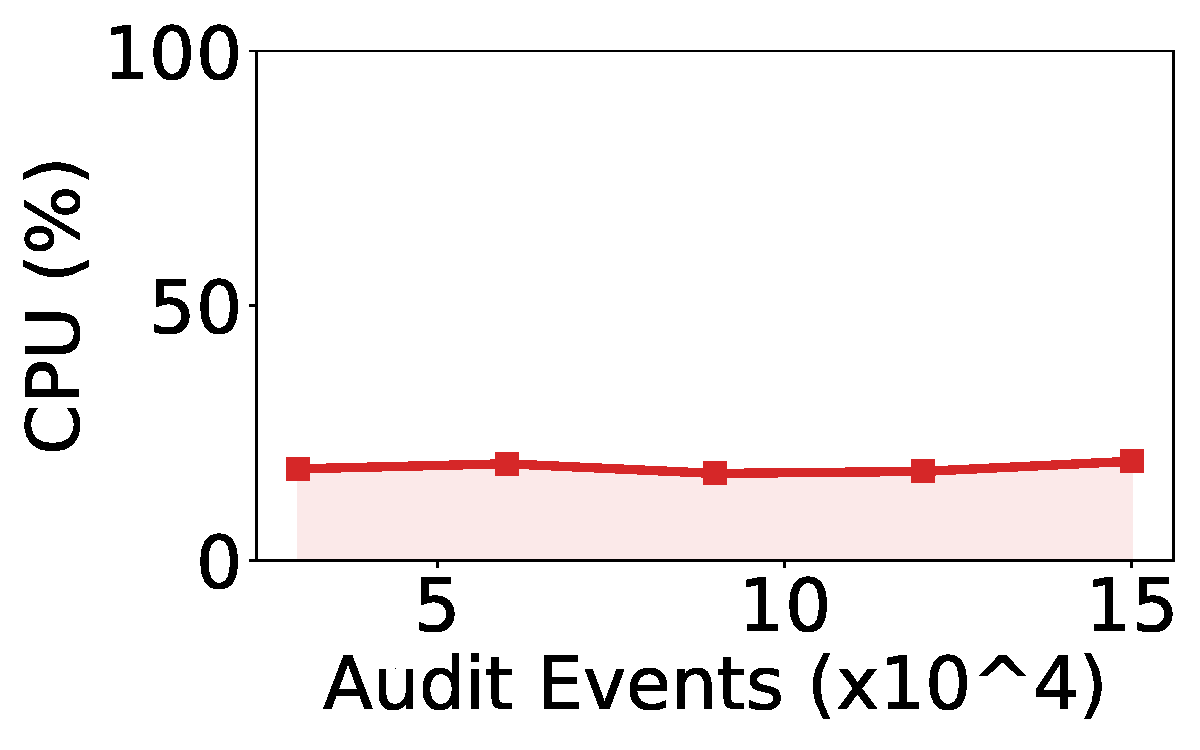
\includegraphics[width=0.24\textwidth]{fig/cpu.pdf}\label{cpu_client}}
  \hfill
  \subfloat[RAM utilization client side]{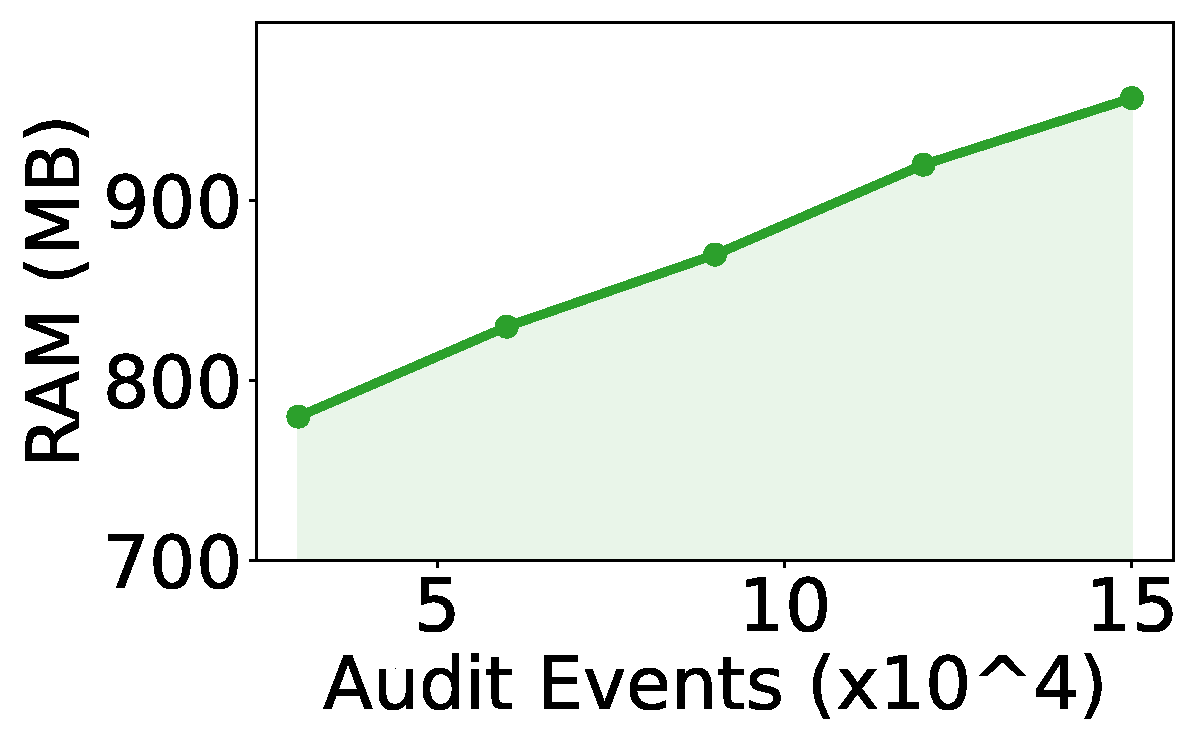
\includegraphics[width=0.24\textwidth]{fig/ram.pdf}\label{ram_client}}
  \hfill
  \subfloat[CPU utilization central server.]{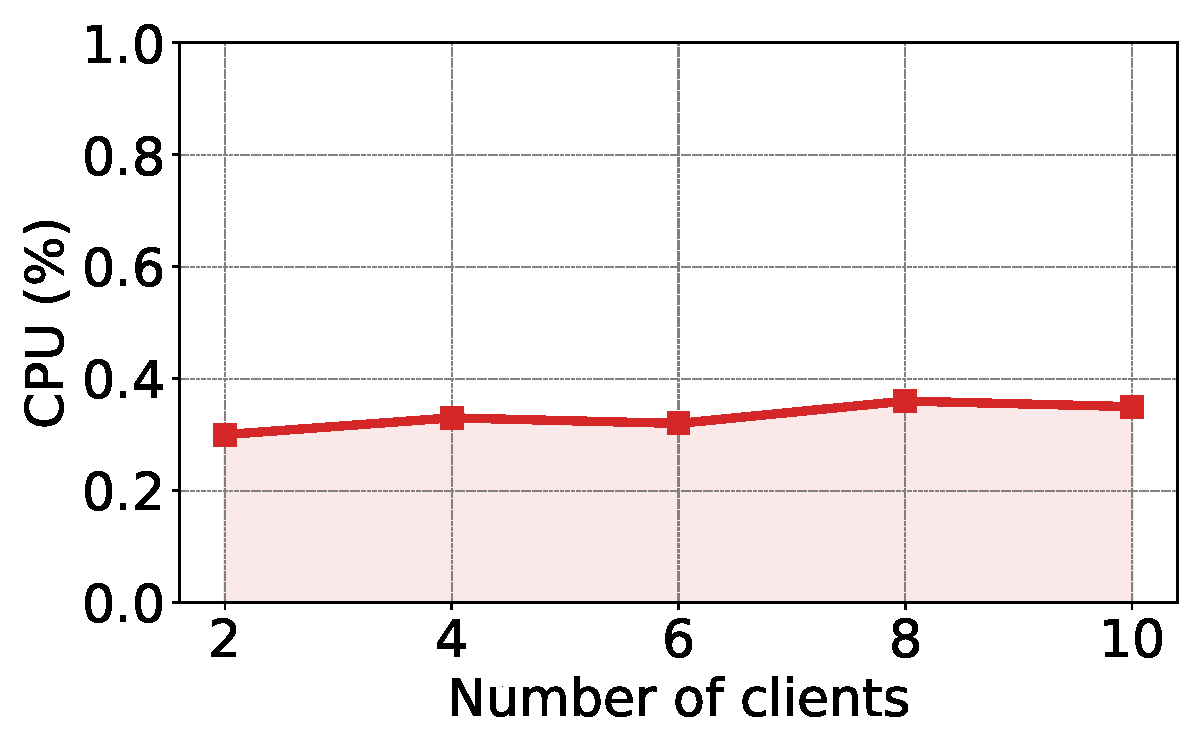
\includegraphics[width=0.24\textwidth]{fig/cpu_central.pdf}\label{cpu_central}}
  \hfill
  \subfloat[RAM utilization central server]{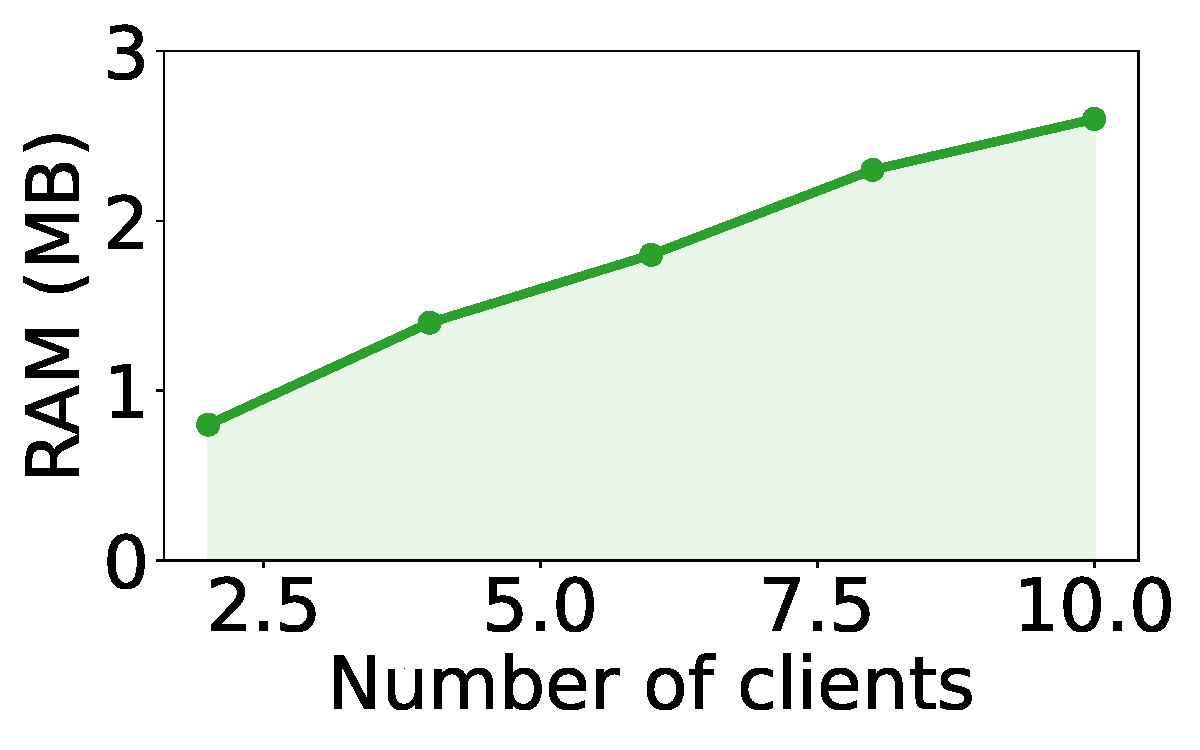
\includegraphics[width=0.24\textwidth]{fig/ram_central.pdf}\label{ram_central}}
  \hfill
  \subfloat[CPU utilization utility server.]{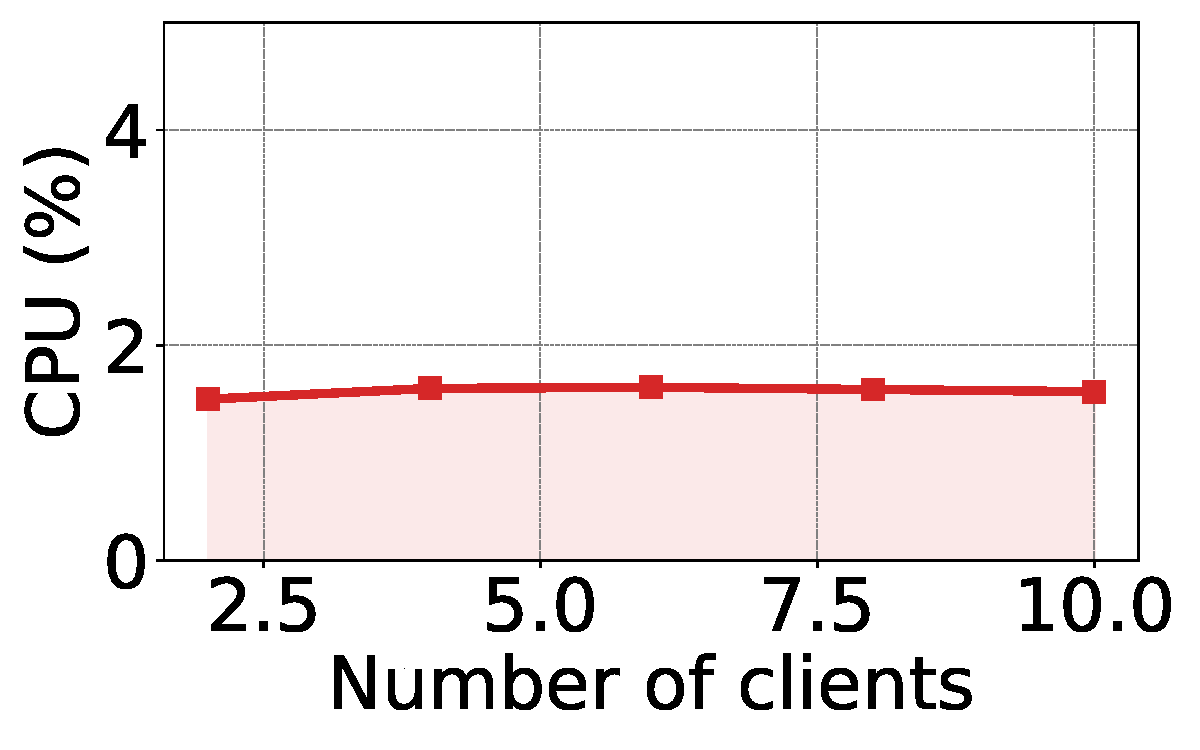
\includegraphics[width=0.24\textwidth]{fig/cpu_utility.pdf}\label{cpu_utility}}
  \hfill
  \subfloat[RAM utilization utility server]{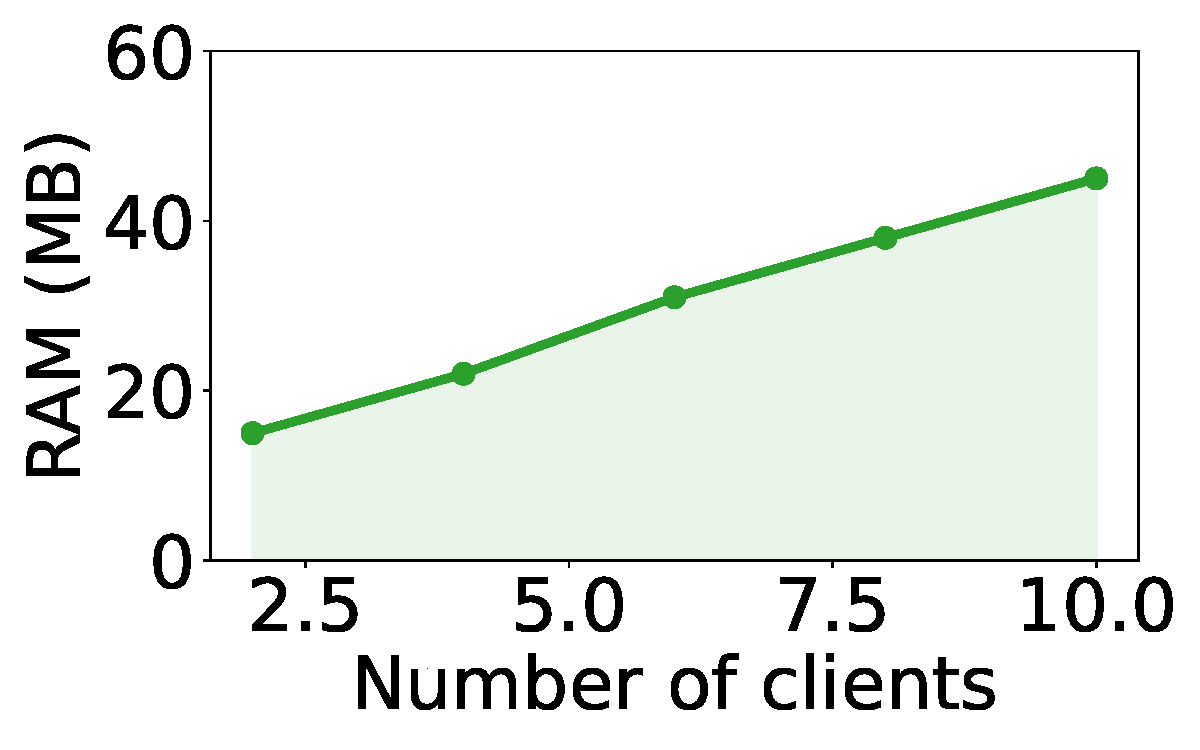
\includegraphics[width=0.24\textwidth]{fig/ram_utility.pdf}\label{ram_utility}}
  \caption{Resource consumption of various components of \Sys.}
  \label{fig:resource}
  \vspace{-2ex}
\end{figure}

\PP{Processing Time Analysis} We conducted experiments to study the end-to-end processing time of our system for a client machine. For this, we used batches of audit events of various sizes, conducting end-to-end inference with \Sys to measure the time taken to process these events on a client machine. The results, illustrated in Figure~\ref{sizevstime}, demonstrate that \Sys processes events with notable efficiency. For example, it requires approximately 23 seconds to process a batch of 100,000 events. Given our previous analysis of host logs in the \optc dataset, which indicated that each host generates an average of 100,000 events in three hours, \Sys can process 24 hours worth of log data on a client in merely 3 minutes. This level of efficiency ensures that our system is highly effective, preventing any potential log congestion.

\begin{figure}[!h]
  \centering
  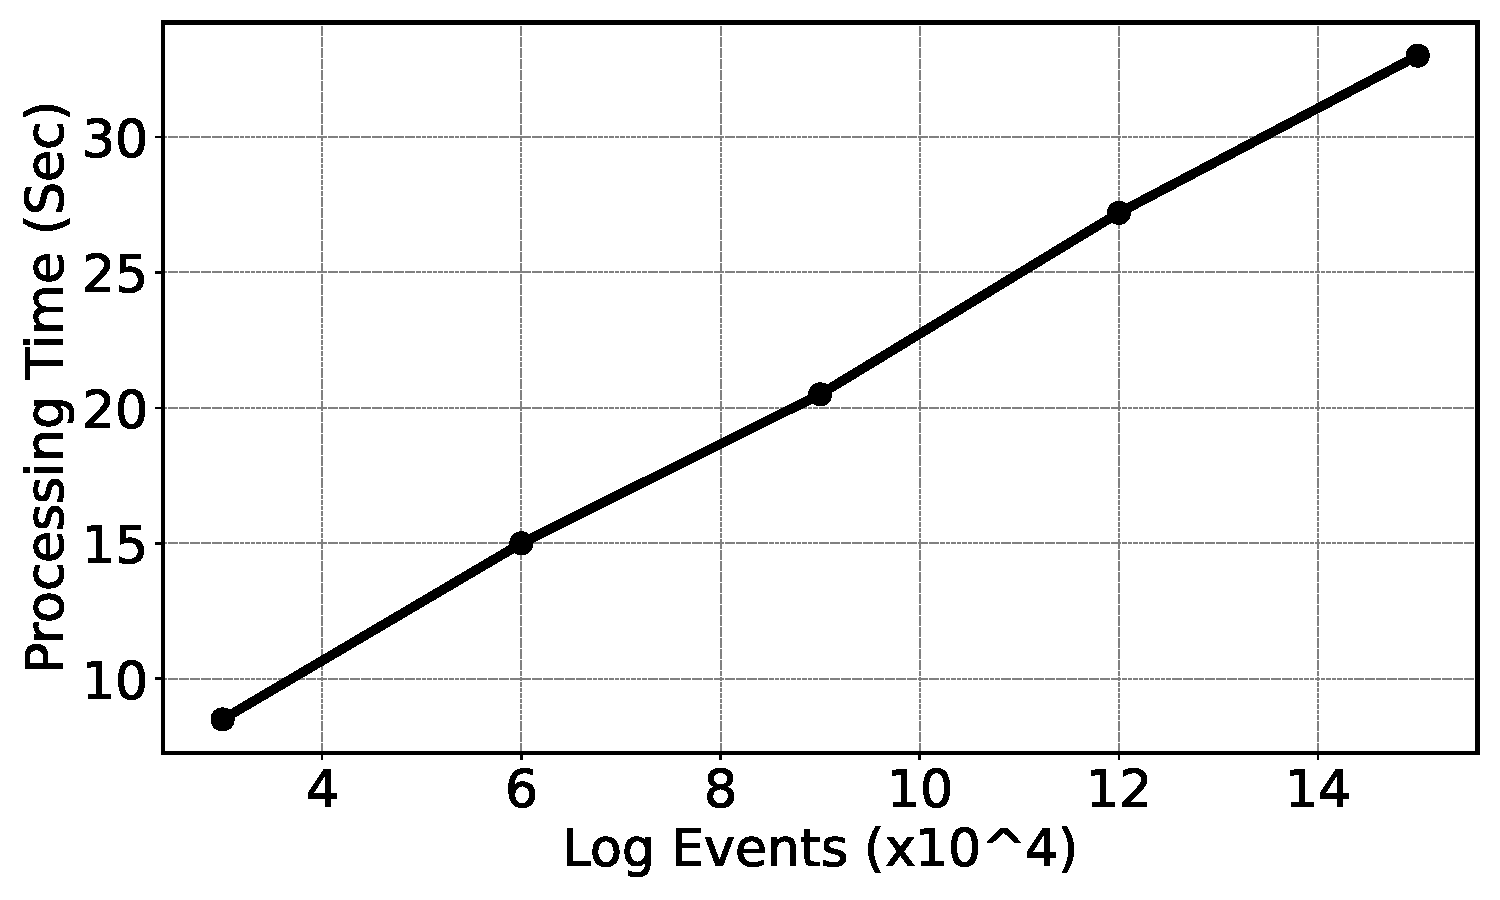
\includegraphics[width=0.35\textwidth]{fig/sizevstime.pdf}
  \caption{Processing time for various audit event sizes evaluated using \optc dataset. }
  \label{sizevstime}
  \vspace{-2ex}
 \end{figure}


\section{RQ7: Ablation study}
\label{app:ablation}

In this ablation study, we analyze the impact of key parameters within \Sys. Specifically, we examine the effects of number of federated averaging rounds, the number of \gnnshort categorized models, the anomaly threshold and differential privacy on accuracy. The effects of these parameters are discussed below:

% \PP{Hosts vs Detection Performance} We utilized the \optc dataset for this experiment, randomly selecting a variable number of hosts to participate in training our models through federated learning. The trained global models were then applied to perform threat detection. Figure~\ref{scoresvshosts} presents these results, illustrating that performance improvement is observed up to a certain number of hosts. This plateau is attributed to the \optc dataset's finite set of benign patterns that can be learned. Beyond this threshold, additional hosts do not contribute new information beneficial to the model, thus halting further performance gains and increasing the risk of overfitting. To mitigate this, client machines can monitor the loss of the global model on their local datasets to determine the optimal point to opt out from the learning process.

% \begin{figure}[!t]
%   \centering
%   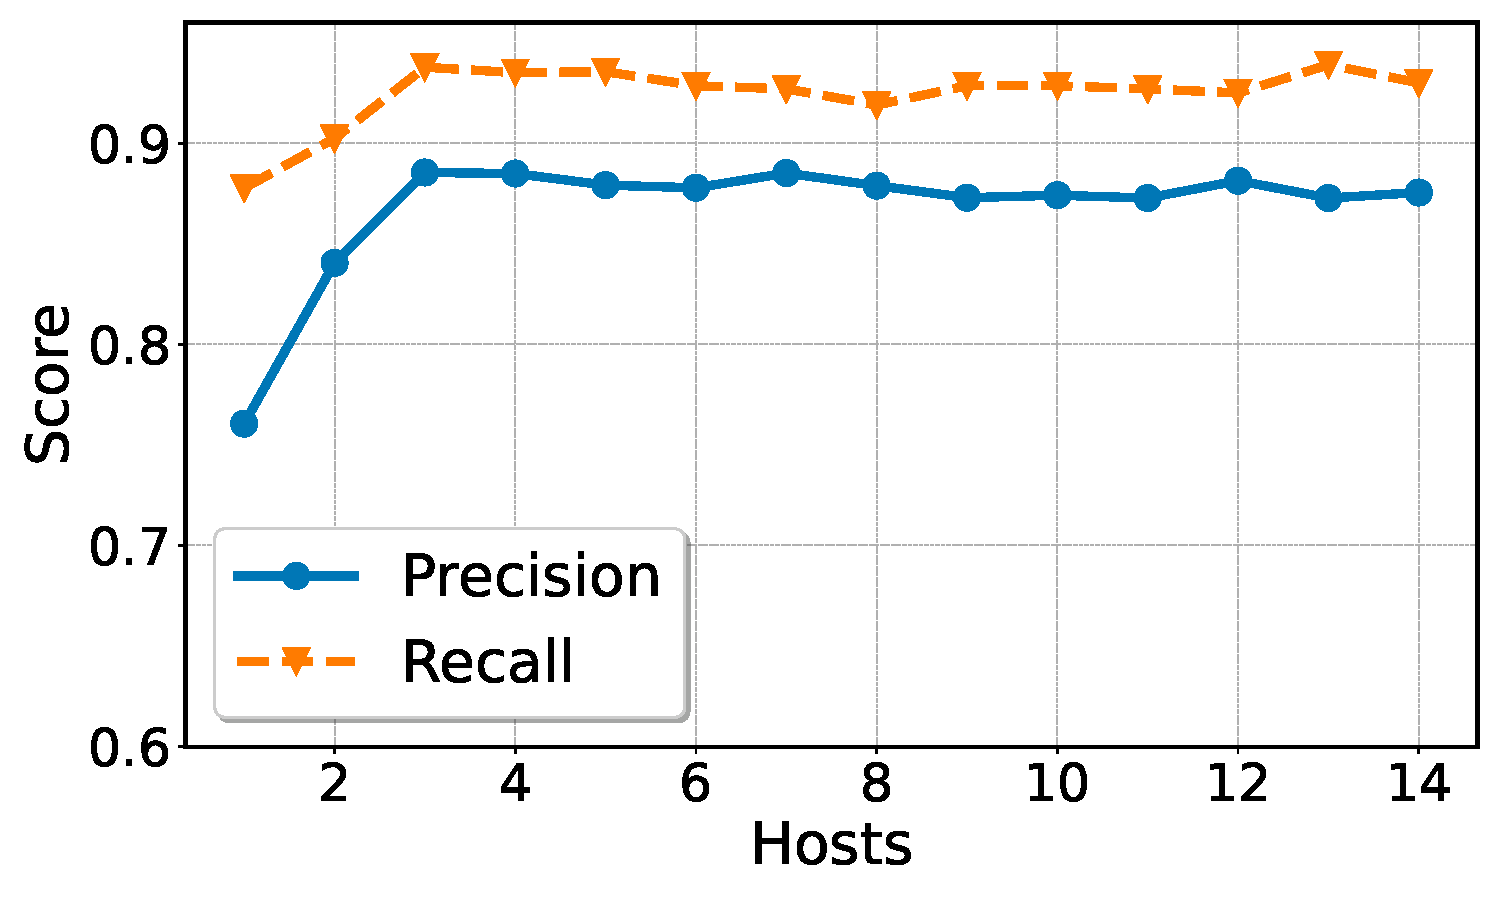
\includegraphics[width=0.3\textwidth]{fig/scoresvshosts.pdf}
%   \caption{Effect of number of hosts vs detection metrics using \optc dataset.}
%   \label{scoresvshosts}
%   \vspace{-2ex}
% \end{figure}


\subsection{Effectiveness of \wordvec harmonization}
\label{sub:word2vec:harmonization:efficacy}

We evaluated the effectiveness of our \wordvec vector harmonization scheme through two experiments using the \optc, E3 and E5 datasets. In the first experiment, each client utilized its locally trained \wordvec model to encode semantic features during the training process. In the second experiment, we harmonized the individually trained models into a central \wordvec model using the utility server architecture, as explained in Section~\ref{sec:methodology}. Then each client used this centralized model for generating semantic features. Table~\ref{local:wordvec} presents the average results for the \darpa E3, E5 and \optc datasets. By employing the harmonized models, we achieved significantly better detection outcomes. This is because these local models encode different information for identical tokens across hosts. Such variability leads to heterogeneity in the feature space for the \gnnshort model, impairing the model's ability to generalize and converge effectively during the federated learning process, thereby yielding suboptimal results. However, through our novel, privacy-preserving aggregation of these semantic models, we have addressed this issue by merging the information in these models together to give the \gnnshort more generalized input vectors.


\begin{table}[!h]
 \centering
 \small
 \setlength{\tabcolsep}{10pt}
 \caption{Effectiveness of \wordvec harmonization.}
 \begin{tabular}{ | c | c | c | c | c |}
   \hline
   \bf Dataset & \bf Type & \bf Prec. & \bf Rec. & \bf \fscore \\
   \hline
   \multirow{2}{*}{\optc} & Local & \VFOP & \VFOR & \VFOF \\
   \cline{2-5}
   & Harmonized & \TOP & \TOR & \TOF \\
   \hline
   \multirow{2}{*}{E3} & Local & 0.83 & 0.96 & 0.89 \\
   \cline{2-5}
   & Harmonized & 0.96 & 0.99 & 0.97 \\
   \hline
   \multirow{2}{*}{E5} & Local & 0.81 & 0.94 & 0.87 \\
   \cline{2-5}
   & Harmonized & 0.98 & 0.98 & 0.98 \\
   \hline
 \end{tabular}
 \label{local:wordvec}
\end{table}

\subsection{Effectiveness of categorized graph learning}
\label{sub:categorized:learning:efficacy}

%\wajih{let's divide this RQ into two RQs and update the first paragraph of the evalution section. Also, please move Word2vec harmonization before Categorization as they are in the design seection.}

To examine the effectiveness of our process categorization based \gnnshort ensemble technique, we conducted experiments comparing our ensemble technique against a single model approach in a federated setting. Specifically, for the ensemble method, we designated the number of categories to be 10. This approach standardizes all processes across various hosts into 10 distinct categories, ensuring that the \gnnshort models learn similar distributions regardless of the host. Such standardization is crucial for mitigating the impact of heterogeneous distributions and data imbalance during the federated averaging process. Table~\ref{categorized_gnn} reports the average results for the \darpa E3, E5 and \optc datasets. The results indicate that utilizing categorized ensemble models yields superior performance. This improvement is attributed to each sub-model's enhanced ability to concentrate on different patterns of system activity from different clients, thereby reducing the likelihood of these patterns becoming conflated during the federated averaging process. We also studied the effect of different number of categories on detection accuracy in Appendix~\ref{app:categories}.%\wajih{Explain the reason that why you ignored E5 here. This is a simple way a reviewer can kill your paper as you are trying to hide information.}

% \begin{table}[!t]
%   \centering
%   \small
%   \setlength{\tabcolsep}{10pt}
%   \caption{Effectiveness of categorized \gnnshort learning.}
%   \begin{tabular}{ | c | c | c | c | c |}
%     \hline
%     \bf Dataset & \bf Type & \bf Prec. & \bf Rec. & \bf \fscore \\
%     \hline
%     \multirow{2}{*}{E3-Cadets} & Single & \STCP & \STCR & \STCF \\
%     \cline{2-5}
%     & Ensemble & \TCP & \TCR & \TCF \\
%     \hline
%     \multirow{2}{*}{E3-Trace} & Single & \STTP & \STTR & \STTF \\
%     \cline{2-5}
%     & Ensemble & \TTP & \TTR & \TTF \\
%     \hline
%     \multirow{2}{*}{E3-Theia} & Single & \STTHP & \STTHR & \STTHF \\
%     \cline{2-5}
%     & Ensemble & \TTHP & \TTHR & \TTHF \\
%     \hline
%     \multirow{2}{*}{\optc} & Single & \STOP & \STOR & \STOF \\
%     \cline{2-5}
%     & Ensemble & \TOP & \TOR & \TOF \\
%     \hline
%   \end{tabular}
%   \label{categorized_gnn}
% \end{table}

\begin{table}[!h]
 \centering
 \small
 \setlength{\tabcolsep}{10pt}
 \caption{Effectiveness of categorization-based ensemble learning.}
 \begin{tabular}{ | c | c | c | c | c |}
   \hline
   \bf Dataset & \bf Type & \bf Prec. & \bf Rec. & \bf \fscore \\
   \hline
   \multirow{2}{*}{\optc} & Single & \STOP & \STOR & \STOF \\
   \cline{2-5}
   & Ensemble & \TOP & \TOR & \TOF \\
   \hline
   \multirow{2}{*}{E3} & Single & 0.89 & 0.99 & 0.94 \\
   \cline{2-5}
   & Ensemble & 0.96 & 0.99 & 0.97 \\
   \hline
   \multirow{2}{*}{E5} & Single & 0.92 & 0.96 & 0.94 \\
   \cline{2-5}
   & Ensemble & 0.98 & 0.98 & 0.98 \\
   \hline
 \end{tabular}
 \label{categorized_gnn}
\end{table}


\subsection{Effect of federated averaging rounds}
\label{app:fedrounds}

We employed the \darpa E3 dataset to examine the impact of federated averaging rounds on detection performance. Our methodology involved training the model over a range of federated averaging rounds and subsequently evaluating the model's detection capabilities. The outcomes are depicted in Figure~\ref{roundsvsscore}, which shows that detection performance improves up to a certain number of rounds before declining due to overfitting. Notably, this inflection point is also characterized by a minimal decrease in training loss, suggesting that the model has reached its learning capacity. This observation proves to be a valuable metric for determining the optimal moment to stop training, thereby preventing overfitting and ensuring optimal model performance. 

\begin{figure}[!t]
  \centering
  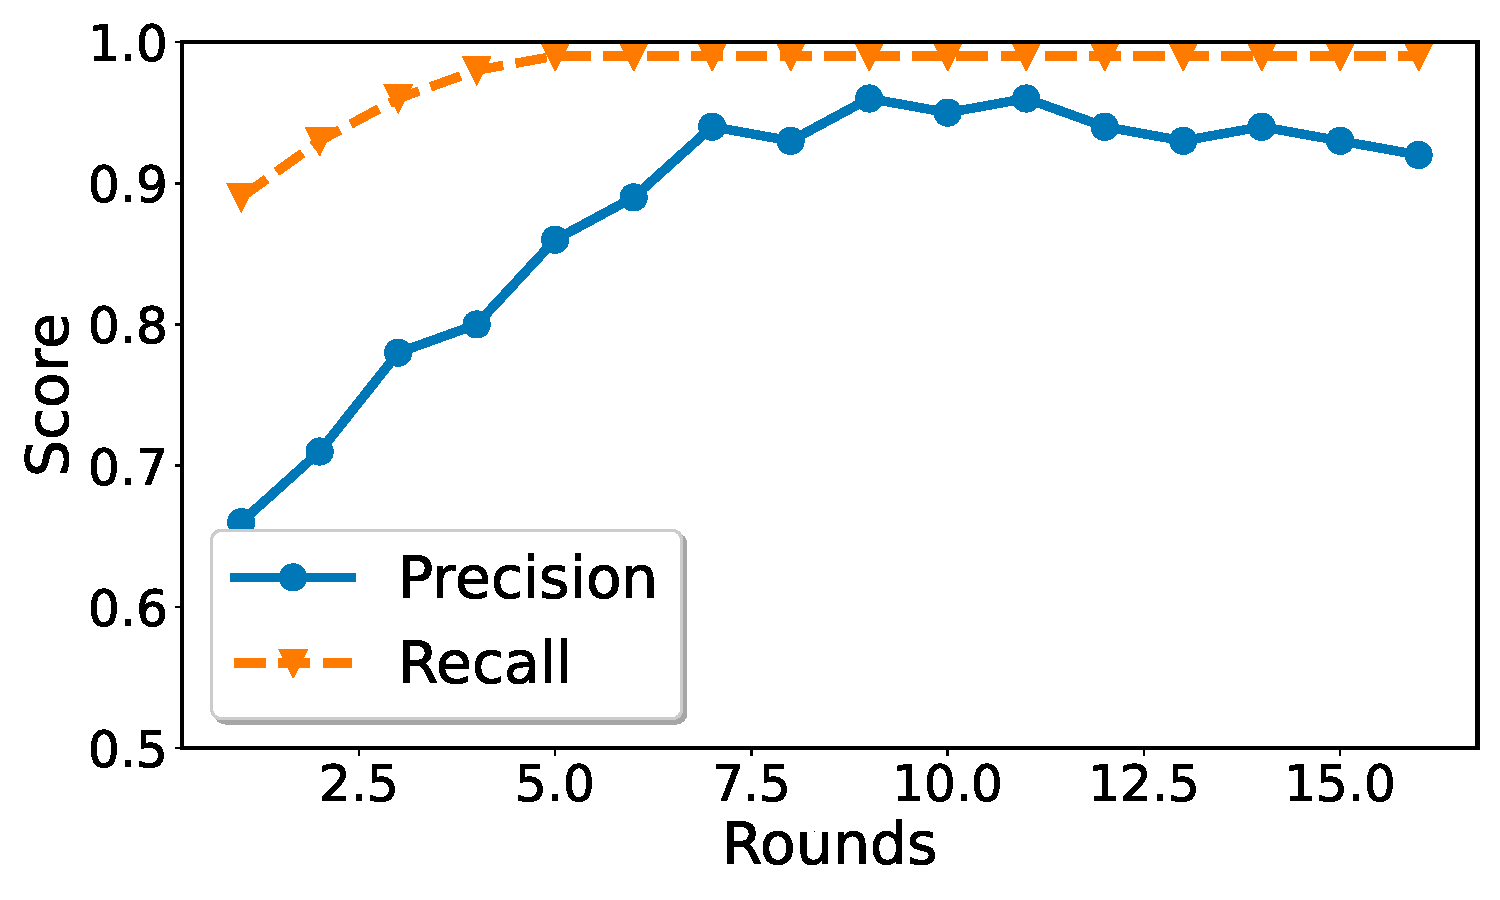
\includegraphics[width=0.35\textwidth]{fig/roundsvsscore.pdf}
  \caption{Federated averaging rounds vs detection performance using E3 dataset.}
  \label{roundsvsscore}
  \vspace{-2ex}
\end{figure}

\subsection{Effect number of categories vs detection}
\label{app:categories}

We studied the impact of varying the number of categories ($k$) on the detection performance. Within our system entity-level \gnnshort learning framework, $k$ controls the creation of distinct standardized bins. These bins categorize processes across client machines. Subsequently, we employ an ensemble approach, deploying a separate \gnnshort model for each bin. Thus, the total number of \gnnshort models corresponds to the number of categories. The results depicted in Figure~\ref{catgvsscore} indicate that an increase in $k$ enhances precision while maintaining recall levels. This outcome arises because a single model suffices for achieving high recall by effectively distinguishing between benign and malicious patterns. Nevertheless, a single model falls short in fully generalizing across the diverse benign patterns unique to each client due to the potential blending of individual patterns during the process of federated averaging. Employing a specialized \gnnshort strategy across various categories addresses this challenge by minimizing false alarms.

\begin{figure}[!h]
  \centering
  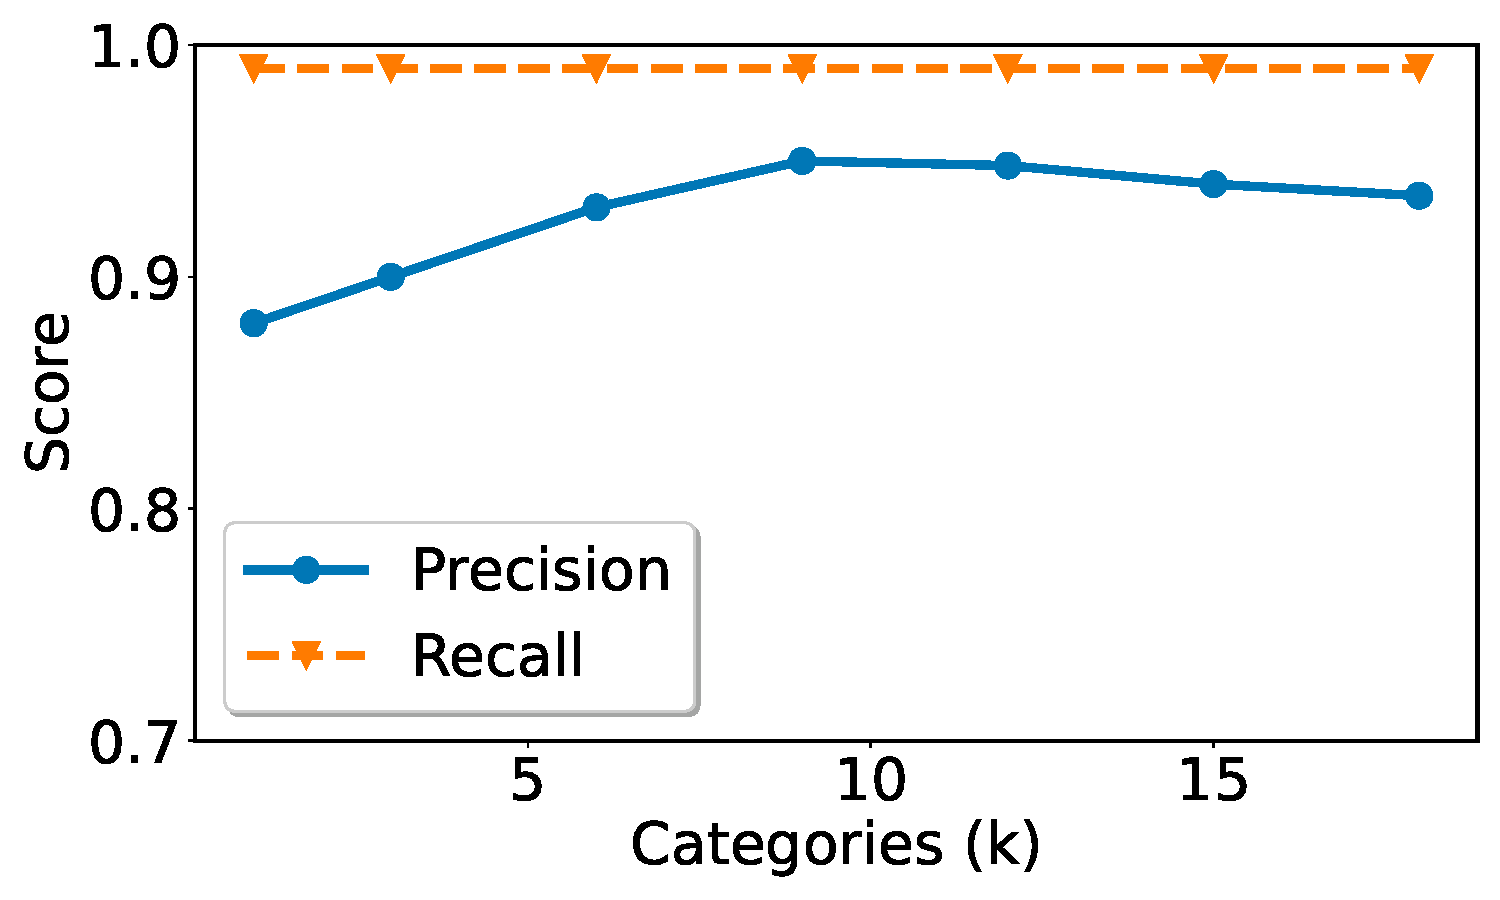
\includegraphics[width=0.35\textwidth]{fig/kvsscore.pdf}
  \caption{Effect of number of categories vs detection performance using E3 dataset.}
  \label{catgvsscore}
  \vspace{-2ex}
\end{figure}

\subsection{Effect number of categories on training cost}
\label{app:traincost}

We analyzed the impact of the number of submodels on the training costs in FL. The training cost is influenced by two primary factors: the time required to train a \gnnshort model on a single client machine and the network overhead incurred from communicating multiple models. Our analysis of these factors revealed that each \gnnshort model in the ensemble is consistently 13kb, a size that is determined by the model architecture and does not vary across different datasets. According to our ablation study~\ref{app:categories}, the optimal number of categories is 10, suggesting that the impact on network overhead is minimal. Furthermore, the overall training cost remains unaffected since the total amount of data does not change; it is merely divided into different groups. This division actually enhances the training process by enabling parallel training of the models, highlighting the efficiency of our technique. Therefore, the training duration for our ensemble model is primarily limited by the time required to train the submodel managing the largest data bin.

%\subsection{Detection Performance Under Different Methods}

%\wajih{In the Nature's paper they apply different federated learning and GNN approaches to show that the one they propose is best. I remember you tried different FL approaches as well. Also tried if you can replace GNN with something else. In our Flash paper we have something similar where we switched ML methods to show the performance. I would like to see similar experimentation here as well. The idea is to prove that the method that we chose is the best.}

% \PP{Effect of number of clients on scalability} \Sys operates in a decentralized manner, ensuring that its scalability post-deployment is independent of the client machines count. After the \fpgl phase concludes, each client runs \Sys locally. However, the number of clients may affect scalability during the training phase, potentially impacting the central and utility servers. The primary function of the central server is to conduct federated averaging on model weights from clients—a straightforward matrix mean operation that requires minimal resources, even with thousands of matrices. Similarly, the utility server's role is to sum and average vectors for overlapping semantic attributes, a task that modern machines are optimized to perform for a large number of samples. Importantly, these operations occur solely during the training phase and do not impact the scalability of the deployed system.

\subsection{Anomaly threshold}
\label{app:threshold}

This hyperparameter controls the number of alerts generated by \Sys. It determines the trade-off between precision and recall. We use the E5 dataset to investigate the effects of different anomaly thresholds. Figure~\ref{thresh} illustrates the results. \wajih{add more details here. }

\begin{figure}[!h]
  \centering
  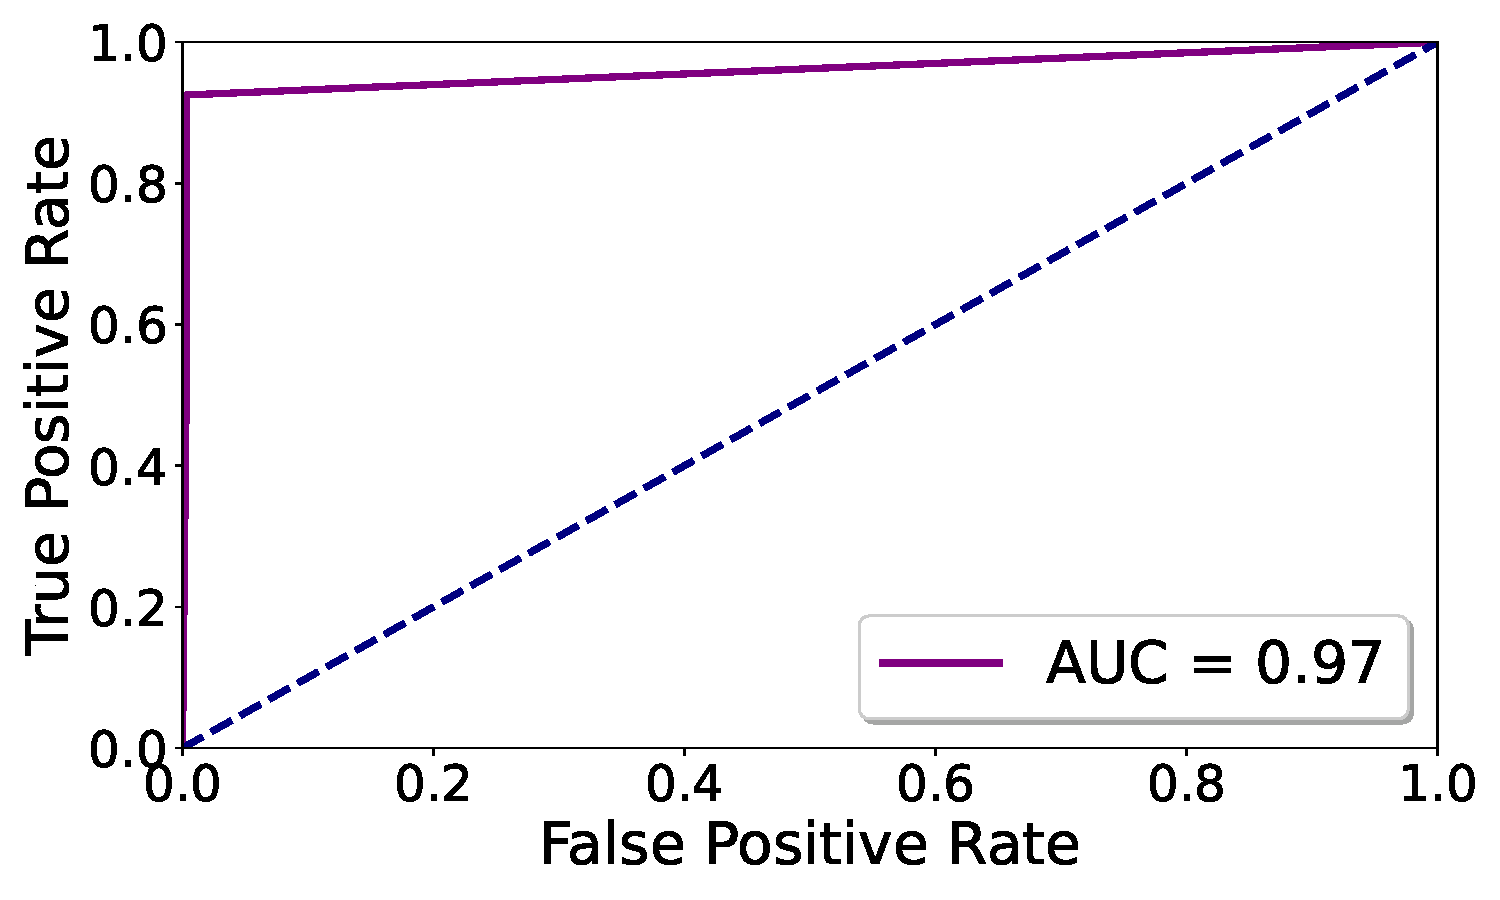
\includegraphics[width=0.35\textwidth]{fig/thresh.pdf}
  \caption{Anomaly threshold effect.}
  \label{thresh}
  \vspace{-2ex}
\end{figure}


\section{Comparison of encryption methods}
\label{app:encrypt}

We chose Fernet symmetric key encryption for its ability to efficiently handle large datasets while ensuring confidentiality and integrity. Fernet employs AES-based symmetric encryption along with an HMAC for authenticity. Because the HMAC relies on efficient hash functions rather than expensive asymmetric operations~\cite{raj2023performance}, Fernet is computationally more efficient for processing large volumes of data.

In contrast, asymmetric methods like RSA which use public-private key pairs and are commonly employed for key exchange are significantly slower and therefore unsuitable for encrypting large datasets~\cite{menezes2018handbook}. Their computational overhead makes them impractical for scenarios involving substantial data, such as \wordvec models with thousands of tokens.

This efficiency is crucial in \Sys, where we encrypt \wordvec models that can contain a large number of tokens. In our experiments, encrypting and decrypting a \wordvec model with 1000 tokens took Fernet only 0.11 ms, compared to 0.64 ms with RSA, making Fernet nearly six times faster.

After encryption, the utility server harmonizes these encrypted models by performing mean averaging on the vectors of overlapping tokens. It identifies such overlaps, averages their vectors, and updates the model accordingly before returning it to the clients.

Our design ensures privacy without resorting to Homomorphic Encryption (HE). Although HE allows computations directly on encrypted data, it imposes a significant performance penalty~\cite{naehrig2011can}. Its mathematically complex operations reduce throughput and scalability. By avoiding HE, we maintain strong privacy protections without incurring the prohibitive computational costs that would impede efficient real-time model updates.

\section{Effect of differential privacy on accuracy}
\label{app:dp}

In Section~\ref{sec:privacy}, we analyze how our system design offers strong guarantees against model inference attacks. Here we discuss another alternative technique for preserving privacy through the use of Differential Privacy (DP). It can be integrated with federated learning to protect against inference attacks~\cite{lyu2020threats,nasr2019comprehensive,zari2021efficient}, though it comes at the cost of detection accuracy.

Differential privacy safeguards the model by injecting a controlled amount of Gaussian noise into its parameters, thereby concealing the influence of any individual data point. In our work, we adopt a node-level DP strategy, which ensures that each node’s features and labels are protected when noise is added to the gradient updates. As a result, individual node contributions remain obscured in the aggregated model parameters, reducing the likelihood of identifying specific nodes or their features. We conduct experiments to examine how varying levels of differential privacy noise affect the detection performance of \Sys. The noise is adjusted based on a privacy budget defined by~$\epsilon$. This noise is applied to local \gnnshort model updates before they are aggregated at the central server during federated averaging, as described in Section~\ref{sec:methodology}.

\begin{figure}[!t]
  \centering
  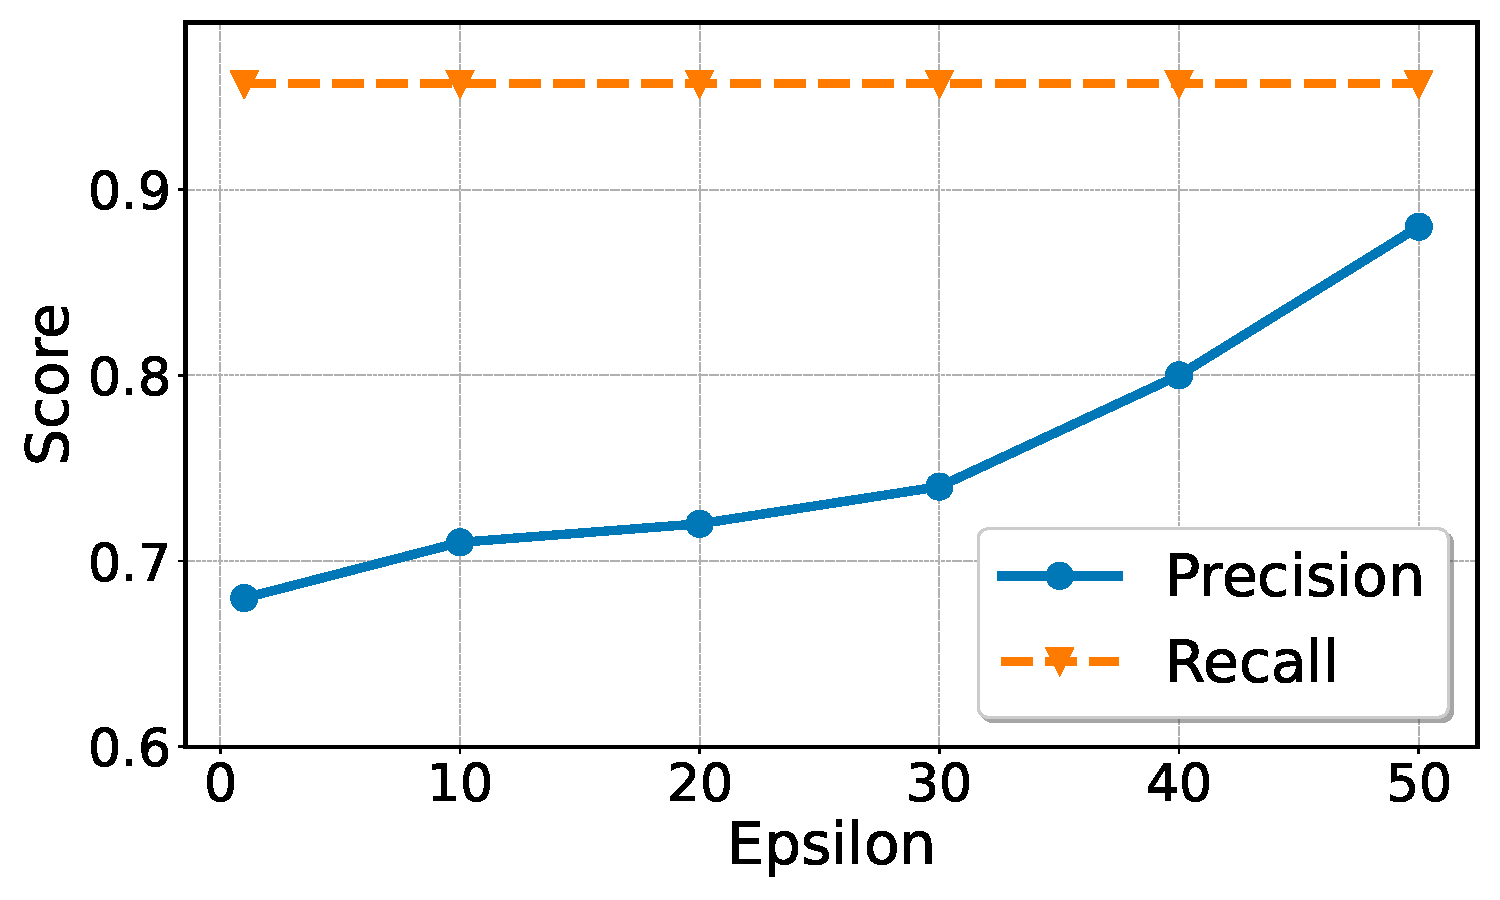
\includegraphics[width=0.3\textwidth]{fig/epsvsscore.pdf}
  \caption{Effect of differential privacy noise on detection using E3 dataset. Note that we observed similar results on the other datasets.}
  \label{epsvsscore}
  \vspace{-2ex}
\end{figure}


The privacy budget~$\epsilon$ plays a pivotal role. Lower values of $\epsilon$ increase the noise injected into the model, which enhances privacy at the expense of detection performance. Conversely, higher values of $\epsilon$ inject less noise, improving detection accuracy but offering weaker privacy guarantees. By tuning $\epsilon$ during training, we explore the balance between privacy and detection effectiveness across various settings. As shown in Figure~\ref{epsvsscore}, increasing the noise level (i.e., reducing $\epsilon$) degrades the model’s utility, thereby providing more privacy at the cost of lower accuracy.

Hence, although DP is a valid solution for protecting privacy, the accuracy deterioration that comes with it reduces its utility in the domain of intrusion detection, where high detection performance is needed. Due to these reasons, we do not use DP in \Sys and instead design a dual-server architecture to offer privacy guarantees without adding noise to the model updates.

% \section{State Explosion in Massive Networks}
% \label{state:explosion}

% Scaling FL to larger enterprise networks introduces potential state explosion issues, primarily due to the increasing complexity in managing and integrating updates from a growing number of clients. As more clients participate, each contributing their local model updates, the volume of data to be processed and aggregated can increase significantly. This escalation can strain communication channels, leading to higher bandwidth requirements and increased latency. Furthermore, the aggregation process itself becomes more computationally demanding as the number of updates grows. \Sys addresses these challenges by utilizing an ensemble learning approach and categorizing system activities, which simplifies the aggregation by processing more uniform data segments. Moreover, our system uses models with small network overhead to prevent bandwidth challenges. To further enhance efficiency, additional techniques such as model compression~\cite{choudhary2020comprehensive}, selective update aggregation~\cite{ye2020federated} and the implementation of more robust communication protocols~\cite{laclau2020robust} can significantly improve handling large volumes of updates, thus preventing state explosion and maintaining system performance in large-scale federated learning environments.


% \section{Word2vec Semantic Featurization}
% \label{app:Word2vec:Semantic:Featurization}
% \label{sub:hyper}

% In  federated learning, where data originates from diverse sources such as user machines running various processes, quantifying this diversity becomes crucial for model development. The Shannon Diversity Index (SDI) is a metric adapted from ecology to measure the heterogeneity of datasets. This report elaborates on the application of SDI in federated learning, focusing on comparing the diversity of sub-models in an ensemble approach to a single model scheme.

% \section*{The Shannon Diversity Index (SDI)}

% SDI quantifies a dataset's diversity by considering both the variety of items (richness) and the distribution frequency of each item (evenness). It is given by:

% \[
% H' = -\sum_{i=1}^{R} p_i \ln(p_i)
% \]

% where:
% \begin{itemize}
%     \item $H'$ is the Shannon Diversity Index,
%     \item $R$ denotes the number of unique items,
%     \item $p_i$ represents the proportion of the dataset made up by the $i$th item.
% \end{itemize}

% In federated learning, SDI can reveal the heterogeneity within the data, guiding the strategy for model training and data segmentation.

% \section*{Application of SDI in Federated Learning}

% \subsection*{Scenario Overview}

% A federated learning setup involves analyzing process data from user machines. This scenario examines the diversity of processes, considering the significant overlap among users.

% \subsection*{Example Dataset}

% The dataset features processes like Chrome, Excel, Spotify, and others, from four user machines. Each machine's processes exhibit a 50\% overlap with others, presenting a realistic view of data distribution.

% \subsection*{Process Distribution Across Users}

% \begin{itemize}
%     \item \textbf{User 1}: \{Chrome, Excel, Spotify, Zoom, Slack\}
%     \item \textbf{User 2}: \{Word, PowerPoint, Teams, Slack, Spotify\}
%     \item \textbf{User 3}: \{Chrome, Zoom, Teams, Excel, Word\}
%     \item \textbf{User 4}: \{PowerPoint, Spotify, Slack, Chrome, Word\}
%     \item \textbf{User 5}: \{Chrome, Zoom, Teams\}

% \end{itemize}

% Processes are then randomly divided into three groups.

% \subsection*{Computing SDI for Each Group and single  Scheme}

% SDI calculations are based on the occurrence frequencies of processes, assessing diversity within each group and comparing it to a single  model approach where all processes are considered together.

% \subsubsection*{SDI Results}

% \begin{itemize}
%     \item \textbf{Category 1}: {Chrome, Zoom, and Teams}.
%     \item \textbf{Category 2}: {Word, Excel, and PowerPoint}.
%     \item \textbf{Category 3}: {Spotify and Slack}.
% \end{itemize}

% \subsection*{Analysis and Implications}

% \begin{itemize}
%     \item \textbf{Category 1 SDI}: $H' = 1.08$
%     \item \textbf{Category 2 SDI}: $H' = 1.10$
%     \item \textbf{Category 3 SDI}: $H' = 0.67$
%     \item The single  model, considering all processes together, yielded an SDI of $H' = 2.06$.
% \end{itemize}

% \subsubsection*{Diversity Comparison}

% Compared to the single  model's SDI, each sub-model reflects a specific aspect of the overall diversity but with reduced complexity, suggesting that sub-models focus on more homogeneous subsets of data.

% \subsubsection*{Influence on Client Fairness}

% By dividing the overall task into sub-tasks (sub-models) and assigning them to different subsets of processes (or data features), the influence of clients with large datasets is diversified across multiple models. This can prevent any single client from disproportionately skewing the outcome of the entire federated learning system.

% \subsubsection*{Balanced Representation}

% Each sub-model specializes in a different aspect of the data, potentially leading to a scenario where clients contribute more evenly across the ensemble. Clients with large datasets still contribute significantly, but their impact is more evenly distributed, enhancing fairness.

% \begin{algorithm}[!t]
%   \scriptsize
%   \DontPrintSemicolon
%   \SetKwInOut{Input}{Inputs}
%   \SetKwInOut{Output}{Output}
%   \Input{Set of client models $\{GNN_1, GNN_2, \ldots, GNN_N\}$;\\}
%   \Output{Global GNN model $GNN_{Global}$.}
%   \BlankLine
%   \tcc{Initialize global GNN model with random weights for a given process Category.}
%   %\tcc{This initialization happens for the first FL round only.}
%   $G \leftarrow \text{InitializeRandomWeights}()$\\
%   \tcc{Distribute $GNN$ to all clients.}
%   \ForEach{client}{
%     Send $GNN$ to $Client_i$\\
%     $GNN \leftarrow \text{TrainOnLocalData}(ProcessCategory_i)$
%   }
%   \BlankLine
%   \tcc{Aggregate trained models from clients.}
%   $AggregatedWeights \leftarrow list([])$\\
%   \ForEach{client model $GNN_i$}{
%     $AggregatedWeights.append(\text{ExtractWeights}(GNN_i))$\\
%   }
%   \tcc{Apply federated averaging.}
%   $GNN_{Global} \leftarrow \text{FederatedAveraging}(AggregatedWeights)$\\
%   \BlankLine
%   \Return $GNN_{Global}$\\
%   \BlankLine
%   \caption{Federated Provenance Graph Learning}
%   \label{alg:federated_learning}
% \end{algorithm}